% !TEX root = ../../main.tex

\section{Approximation de la partie linéaire}
\label{s3:approx}

L'obtention, même à l'aide de calcul ou d'un logiciel de calcul formel, de l'exponentielle de la partie linéaire n'est pas toujours envisageable. Il est possible de recourir à une méthode d'approximation pour obtenir une formulation formelle de celle-ci qui sera possible d'utiliser pour l'écriture du code de simulation. On s'intéressera dans cette section à la partie linéaire $L$ définie par :
$$
  L = \begin{pmatrix}
    0   & -B_0 & 0          &  0          &  \Omega_{pe}^2 & 0             & 0 \\
    B_0 &  0   & 0          &  0          &  0             & \Omega_{pe}^2 & 0 \\
    0   &  0   & 0          &  0          &  0             & \partial_z    & 0 \\
    0   &  0   & 0          &  0          & -\partial_z    & 0             & 0 \\
   -1   &  0   & 0          & -\partial_z &  0             & 0             & 0 \\
    0   & -1   & \partial_z &  0          &  0             & 0             & 0 \\
    0   &  0   & 0          &  0          &  0             & 0             & -v_z\partial_z \\
  \end{pmatrix}.
$$
Cette matrice est de la forme :
$$
  L = \begin{pmatrix}
    A & 0 \\
    0 & -v_z\partial_z
  \end{pmatrix},
$$
dont seul le bloc $A$ pose problème pour calculer formellement l'exponentielle. Ainsi on s'intéressera surtout à la sous-matrice $A$ obtenue après une transformée de Fourier en $z$ du système :
\begin{equation}
  A = \begin{pmatrix}
    0   & -B_0 & 0       &  0       &  \Omega_{pe}^2  & 0             \\
    B_0 &  0   & 0       &  0       &  0              & \Omega_{pe}^2 \\
    0   &  0   & 0       &  0       &  0              & i\kappa       \\
    0   &  0   & 0       &  0       & -i\kappa        & 0             \\
   -1   &  0   & 0       & -i\kappa &  0              & 0             \\
    0   & -1   & i\kappa &  0       &  0              & 0             \\
  \end{pmatrix}
  \label{eq:3:A}
\end{equation}
%Par abus de notation, nous noterons $A_0$, la matrice $A$ pour $\kappa=0$, ce qui revient à une partie linéaire sans les équations de Maxwell, ceci sera utile lors de la comparaison des résultats entre les méthodes.

La matrice $A$ est presque anti-hermitienne, selon les valeurs de $\Omega_{pe}$ (constante liée à des caractéristiques physiques).  Il est nécessaire de trouver une matrice $\Omega$ permettant de transformer $A$ en une matrice anti-hermitienne :
$$
  \Omega = 
  \begin{pmatrix}
    \dmat[0]{\Omega_{pe}^{-1/2},\Omega_{pe}^{-1/2},\Omega_{pe}^{1/2},\Omega_{pe}^{1/2},\Omega_{pe}^{1/2},\Omega_{pe}^{1/2}}
  \end{pmatrix},
$$
où $\Omega$ est obtenu avec les mêmes stratégies qu'un symétriseur. On a alors $A = \Omega^{-1}H\Omega$, avec $H$ une matrice anti-hermitienne :
$$
  H = \begin{pmatrix}
    0           & -B_0         & 0       &  0       &  \Omega_{pe}  & 0           \\
    B_0         &  0           & 0       &  0       &  0            & \Omega_{pe} \\
    0           &  0           & 0       &  0       &  0            & i\kappa     \\
    0           &  0           & 0       &  0       & -i\kappa      & 0           \\
   -\Omega_{pe} &  0           & 0       & -i\kappa &  0            & 0           \\
    0           & -\Omega_{pe} & i\kappa &  0       &  0            & 0           \\
  \end{pmatrix}
$$
donc $H$ est diagonalisable dans une base unitaire : $H = QDQ^{-1}$ où $D$ est une matrice diagonale des valeurs propres de $H$, et $\texttt{sp}(H)\subset i\mathbb{R}$. Cela permet d'assurer que $A$ est également diagonalisable : $A = \Omega^{-1}QDQ^{-1}\Omega = PDP^{-1}$, avec $P=\Omega^{-1}Q$, et on a donc le résultat $\texttt{sp}(A)\subset i\mathbb{R}$. Cela nous permet de déterminer que les valeurs propres de l'exponentielle de $H$ sont sur le cercle unitaire, en effet on a :
$$
  \forall t\in\mathbb{R}, e^{tH} = Qe^{tD}Q^{-1}
$$
avec $Q$ une matrice unitaire, et $D$ la matrice diagonale des valeurs propres, toutes imaginaires pures. On a également pour $A$, $e^{tA}=Pe^{tA}P^{-1}$, ce qui nous permet d'assurer que les valeurs propres de $e^{tA}$ sont sur un cercle, comme l'illustre la figure~\ref{fig:evexpAk}, où les valeurs propres de $e^{A}$ sont calculées numériquement pour différents modes de Fourier $\kappa$.

\begin{figure}
  \centering
  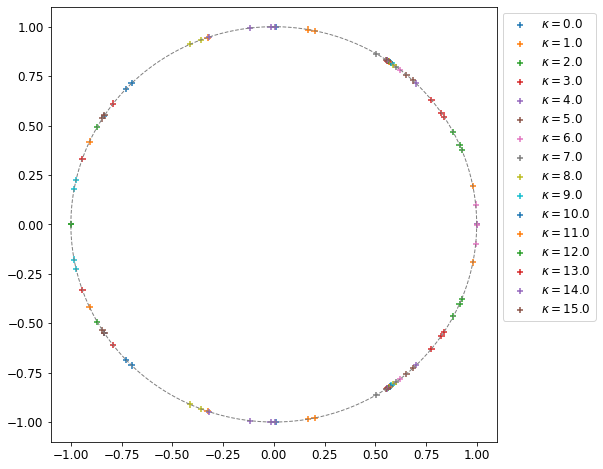
\includegraphics[width=0.5\textwidth]{\localPath/figures/evexpAk.png}
  \caption{Valeurs propres de $e^{A}$ pour différentes fréquences $\kappa\in[\![0,15]\!]$. Les valeurs propres des modes de Fourier négatifs, sont obtenues par parité.}
  \label{fig:evexpAk}
\end{figure}

\subsection{Troncature de la série de Taylor}
%--------------------------------------------------------------------

Un manière classique de définir la fonction exponentielle est par sa série de Taylor, ainsi on définit $e^{tA}$ par :
$$
  e^{M} = \sum_{k=0}^\infty \frac{M^k}{k!}.
$$
Une troncature d'ordre suffisamment élevé $m\geq n$ de cette série permet d'obtenir une approximation de l'exponentielle $e^{tA}$ sans dégrader la méthode LRK($s$,$n$) où elle sera utilisée. Cela garantit que l'erreur de troncature reste supérieure à $n$, l'ordre de la méthode en temps. On définit la troncature de la série de Taylor à l'ordre $m$ par :
$$
  T_m(M) = \sum_{k=0}^m \frac{M^k}{k!}.
$$

Nous savons que les valeurs propres de $e^{tA}$ sont sur le cercle unité, et préserver cette propriété permet d'assurer la stabilité du schéma, par analogie au cas unidimensionnel étudié dans~\cite{Crouseilles:2019b}. Nous regardons donc les valeurs propres de $T_m(A)$ pour $m=\{4,5,6\}$, pour les modes de Fourier $\kappa\in[\![0,15]\!]$ sur les figure~\ref{fig:ev:T4},~\ref{fig:ev:T5} et~\ref{fig:ev:T6}. Le choix $m\leq 4$ se justifie car nous souhaiterons utiliser une méthode de Lawson d'ordre 3 ou 4. On remarque que le module des valeurs propres à 1 n'est pas préservé, quelque soit la valeur de $m$. De plus certaines valeurs propres ont un module très grand, pour $\kappa\geq12$ certaines valeurs propres ont un module supérieur à $10^3$ par exemple. On remarque même que la stabilité pour les petits modes n'est pas assuré, en effet pour $m=6$ (figure~\ref{fig:ev:T6}), aucune valeur propre n'est à l'intérieur du cercle, propriété que semble mieux satisfaire $T_4(A)$ (figure~\ref{fig:ev:T4}).

\begin{figure}
  \begin{subfigure}{.5\textwidth}
    \centering
    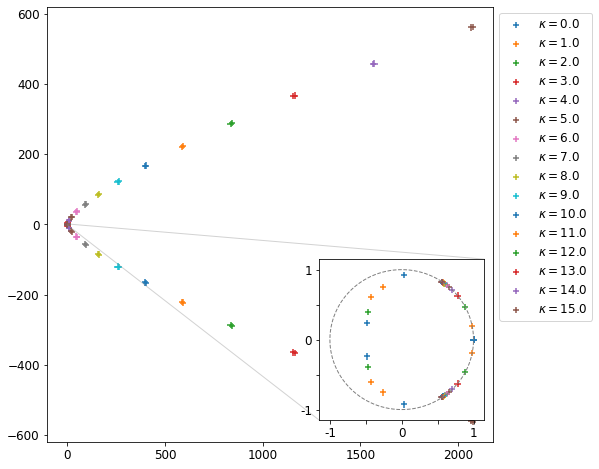
\includegraphics[width=\textwidth]{\localPath/figures/ev_T4.png}
    \caption{Valeurs propres de $T_4(A)$ pour différentes fréquences $\kappa\in[\![0,15]\!]$.}
    \label{fig:ev:T4}
  \end{subfigure}
  \begin{subfigure}{.5\textwidth}
    \centering
    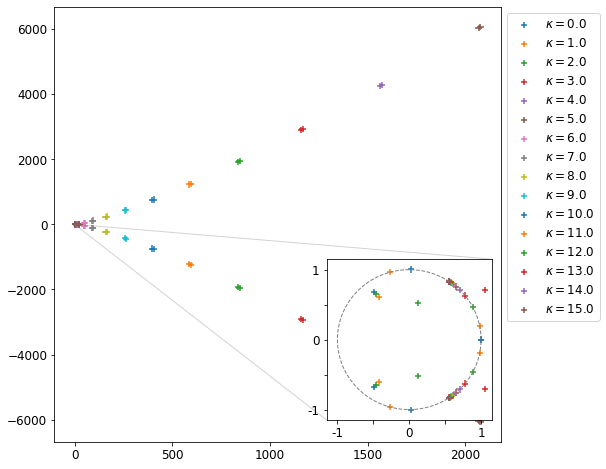
\includegraphics[width=\textwidth]{\localPath/figures/ev_T5.png}
    \caption{Valeurs propres de $T_5(A)$ pour différentes fréquences $\kappa\in[\![0,15]\!]$.}
    \label{fig:ev:T5}
  \end{subfigure}
  \begin{subfigure}{.5\textwidth}
    \centering
    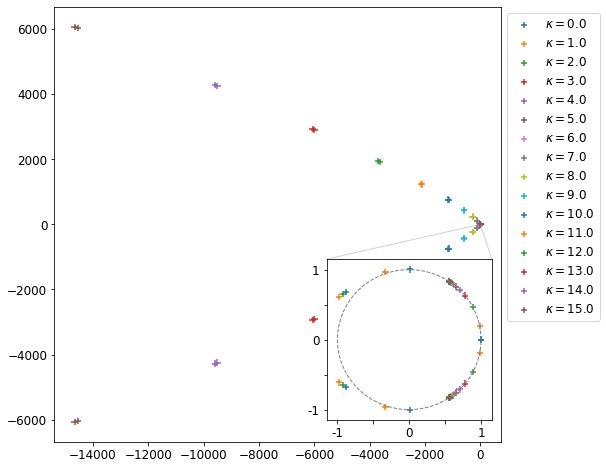
\includegraphics[width=\textwidth]{\localPath/figures/ev_T6.png}
    \caption{Valeurs propres de $T_6(A)$ pour différentes fréquences $\kappa\in[\![0,15]\!]$.}
    \label{fig:ev:T6}
  \end{subfigure}
  \begin{subfigure}{.5\textwidth}
    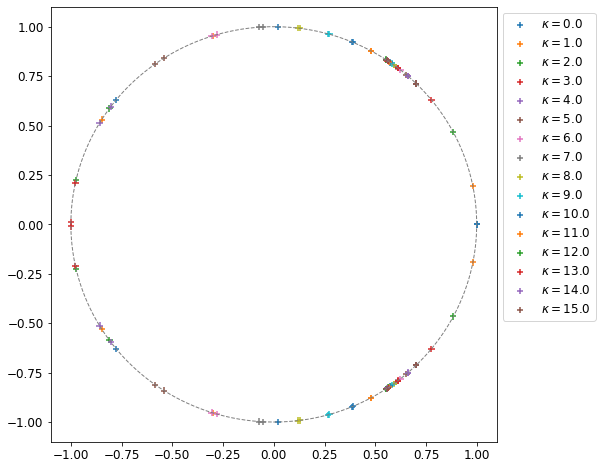
\includegraphics[width=\textwidth]{\localPath/figures/ev_P22.png}
    \caption{Valeurs propres de $P_{2,2}(A)$ pour différentes fréquences $\kappa\in[\![0,15]\!]$.}
    \label{fig:ev:P22}
  \end{subfigure}
  \caption{Valeurs propres de l'approximation de l'exponentielle de $A$ pour différentes fréquences $\kappa\in[\![0,15]\!]$. Les valeurs propres des modes de Fourier négatifs sont obtenues par parité. Les méthodes d'approximation de l'exponentielle de $A$ sont la troncature de Taylor d'ordre 4 ($T_4(A)$) en haut à gauche, la troncature de Taylor d'ordre 5 ($T_5(A)$) en haut à droite, la troncature de Taylor d'ordre 6 ($T_6(A)$) en bas à gauche et l'approximant de Padé d'ordre $(2,2)$ ($P_{2,2}(A)$) en bas à droite.}
\end{figure}



% On peut tracer, pour différentes valeurs de $m$, l'erreur de troncature faite en norme matricielle pour 2 modes de Fourier $\kappa=2$ et $15$, comme le montre la figure~\ref{fig:taylor:error}. Le choix du paramètre $\tau\in[-1,1]$ représente ici le coefficient de Butcher de l'étage considéré, et comme attendu, pour $|\tau|\ll1$ nous observons une bonne précision dans les résultats. L'erreur reste importante, même avec un ordre élevé $m=14$, pour les modes de Fourier plus élevés ($\kappa=15$) lorsque que le paramètre $\tau$ s'écarte de $0$. Ce résultat n'est pas souhaitable, et nous laisse supposer un mauvais comportement de la méthode lors de sa mise en place dans un schéma numérique.

% \begin{figure}
%   \begin{subfigure}{.5\textwidth}
%     \centering
%     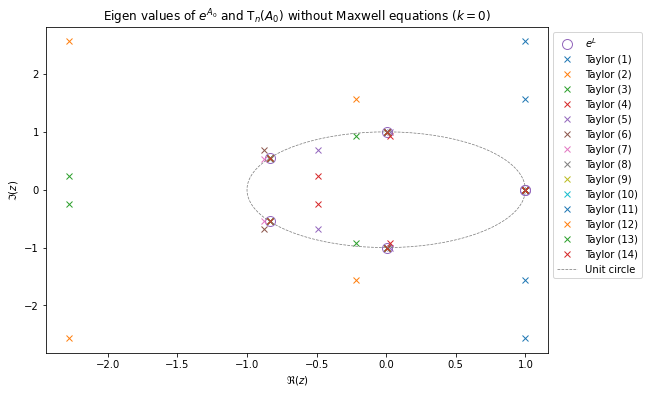
\includegraphics[width=\textwidth]{\localPath/figures/approx_evA0T5.png}
%     \caption{Les valeurs propres de $e^{A_0}$ et de $T_5(A_0)$}
%   \end{subfigure}
%   \begin{subfigure}{.5\textwidth}
%     \centering
%     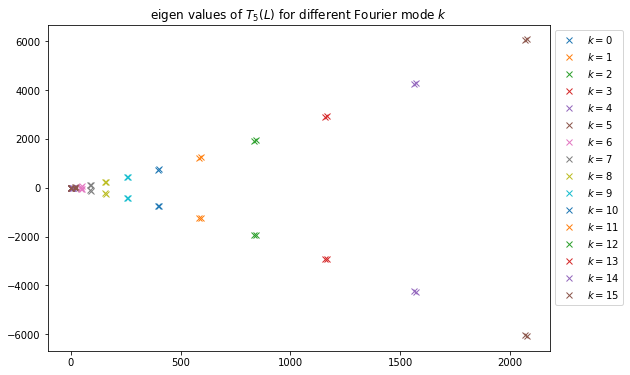
\includegraphics[width=\textwidth]{\localPath/figures/approx_evAkT5.png}
%     \caption{Les valeurs propres de $e^{A}$ et de $T_5(A)$ pour différentes valeurs de $k\in[\![0,15]\!]$, par symétrie on obtient aussi celles pour $k<0$}
%   \end{subfigure}
%   \caption{Valeurs propres de $e^{A}$ et de $T_5(A)$ pour $k=0$ (sans les équations de Maxwell) à gauche, et pour différentes valeurs de $k\in[\![0,15]\!]$ à droite.}
% \end{figure}

% \begin{figure}
%   \begin{subfigure}{.5\textwidth}
%     \centering
%     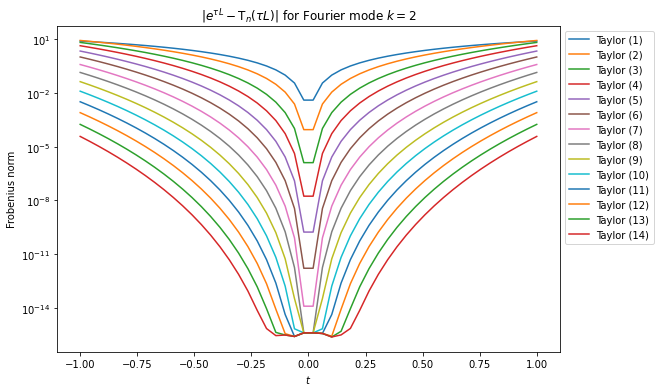
\includegraphics[width=\textwidth]{\localPath/figures/approx_errortA2T.png}
%     \caption{L'erreur absolue locale $\|e^{\tau A}-T_m(\tau A)\|$ pour le mode de Fourier $\kappa=2$}
%   \end{subfigure}
%   \begin{subfigure}{.5\textwidth}
%     \centering
%     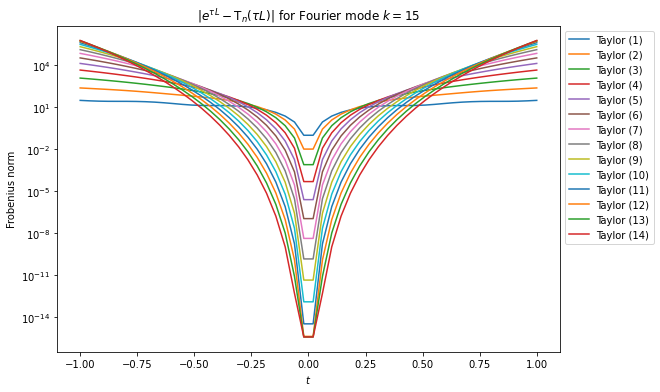
\includegraphics[width=\textwidth]{\localPath/figures/approx_errortA15T.png}
%     \caption{L'erreur absolue locale $\|e^{\tau A}-T_m(\tau A)\|$ pour le mode de Fourier $\kappa=15$}
%   \end{subfigure}
%   \caption{Erreur absolue locale $\|e^{\tau A}-T_m(\tau A)\|$ pour deux modes de Fourier $\kappa=2$ à gauche et $\kappa=15$ à droite.}
%   \label{fig:taylor:error}
% \end{figure}

\subsection{Approximant de Padé}
%--------------------------------------------------------------------

Pour approcher une fonction, au lieu d'utiliser un polynôme comme dans le cadre des séries des développements limités, il est possible de construire une fraction rationnelle. L'approximant de Padé de la fonction exponentielle est la meilleure approximation de la fonction exponentielle par une fraction rationnelle et est définie par :
$$
  \begin{aligned}
    h_{p,q}(x) &= \sum_{i=0}^p \frac{\frac{p!}{(p-i)!}}{\frac{(p+q)!}{(p+q-i)!}}\frac{x^i}{i!} \\
    k_{p,q}(x) &= \sum_{j=0}^q (-1)^j \frac{\frac{q!}{(q-j)!}}{\frac{(p+q)!}{(p+q-j)!}} \frac{x^j}{j!}
  \end{aligned}
$$
$$
  P_{p,q}(x) = \frac{h_{p,q}(x)}{k_{p,q}(x)} \approx e^x
$$
Pour utiliser cet approximant de Padé avec des matrices il faut utiliser la définition suivante :
$$
  e^M \approx P_{p,q}(M) = h_{p,q}(M)\cdot\left(k_{p,q}(M)\right)^{-1}.
$$

L'introduction d'une fraction rationnelle permet de préserver certaines propriétés comme le fait que $P_{p,p}(-z) = \frac{1}{P_{p,p}(z)}$. Nous regardons les valeurs propres de $P_{2,2}(A)$, pour les modes de Fourier $\kappa\in[\![0,15]\!]$ sur la figure~\ref{fig:ev:P22}, et l'on remarque que, contrairement à l'approche basée sur une série de Taylor, le module des valeurs propres est 1, comme pour l'exponentielle exacte.

\begin{pro}
  Pour la matrice $A$ donnée par~\eqref{eq:3:A} :
  $$
    \forall p\in\mathbb{N}_*, \lambda\in\textsf{sp}(P_{p,p}(A)) \implies \lambda\in\mathcal{C}(0,1)
  $$
\end{pro}

\begin{proof}
  Dans un approximant de Padé, lorsque le numérateur et le dénominateur sont de même degré, on peut réécrire l'approximant de Padé comme :
  $$
    P_{p,p}(A) = \left( \sum_{k=0}^p \frac{1}{k!}A^k \right)\cdot\left( \sum_{\ell=0}^p (-1)^\ell\frac{1}{\ell!}A^\ell \right)^{-1}
  $$
  On sait que $A$ est diagonalisable, $A=\Omega^{-1}Q D Q^{-1}\Omega$ avec $D$ une matrice diagonale telle que $\mathsf{sp}(D)\subset i\mathbb{R}$. On réécrit alors l'approximant de Padé $P_{p,p}$ comme :
  $$
    \begin{aligned}
      P_{p,p}(A) &= \left( \Omega^{-1}Q \left( \sum_{k=0}^p \frac{1}{k!}D^k \right) Q^{-1}\Omega \right)
                      \cdot
                    \left( \Omega^{-1}Q \left(\sum_{\ell=0}^p (-1)^\ell \frac{1}{\ell!}D^\ell \right) Q^{-1}\Omega \right)^{-1} \\
                 &= \left( \Omega^{-1}Q \left( \sum_{k=0}^p \frac{1}{k!}D^k \right) Q^{-1}\Omega \right)
                      \cdot
                    \left( \Omega^{-1}Q \left(\sum_{\ell=0}^p (-1)^\ell \frac{1}{\ell!}D^\ell \right)^{-1} Q^{-1}\Omega \right) \\
                 &= \Omega^{-1}Q \left( \sum_{k=0}^p \frac{1}{k!}D^k \right) \cdot \left(\sum_{\ell=0}^p (-1)^\ell \frac{1}{\ell!}D^\ell \right)^{-1} Q^{-1}\Omega
    \end{aligned}
  $$
  La matrice $D$ ayant un spectre imaginaire pur, on note $D = diag\left(\left\{ i\alpha_j, j=1,\dots,6 \right\}\right)$ avec $\alpha_j\in\mathbb{R}$, $j=1,\dots,6$. Cela permet d'expliciter les sommes :
  $$
    \begin{aligned}
      \sum_{k=0}^p \frac{1}{k!}D^k & = diag\left(\left\{ \sum_{k=0}^p i^k\frac{\alpha_j^k}{k!} , j=1,\dots,6 \right\}\right) \\
                                   & = diag\left(\left\{ \sum_{k=0}^{\lfloor\frac{p}{2}\rfloor}(-1)^k\frac{\alpha_j^{2k}}{(2k)!} + i\sum_{k=0}^{\lfloor\frac{p}{2}\rfloor-1}(-1)^k\frac{\alpha_j^{2k+1}}{(2k+1)!} , j=1,\dots,6 \right\}\right) \\
                                   & = diag\left(\left\{ \lambda^+_j , j=1,\dots,6 \right\}\right)
    \end{aligned}
  $$
  De même :
  $$
    \begin{aligned}
      \sum_{\ell=0}^p (-1)^\ell\frac{1}{\ell!}D^\ell & = diag\left(\left\{ \sum_{\ell=0}^p(-i)^\ell\frac{\alpha_j^\ell}{\ell!} , j=1,\dots,6 \right\}\right) \\
                                                     & = diag\left(\left\{ \sum_{\ell=0}^{\lfloor\frac{p}{2}\rfloor}(-1)^\ell\frac{\alpha_j^{2\ell}}{(2\ell)!} - i\sum_{\ell=0}^{\lfloor\frac{p}{2}\rfloor-1}(-1)^\ell\frac{\alpha_j^{2\ell+1}}{(2\ell+1)!} , j=1,\dots,6 \right\}\right) \\
                                                     & = diag\left(\left\{ \lambda^-_j , j=1,\dots,6 \right\}\right)
    \end{aligned}
  $$
  On remarque que $\lambda^+ = \overline{\lambda^-}$. On obtient ainsi :
  $$
    \left( \sum_{k=0}^p \frac{1}{k!}D^k \right) \cdot \left(\sum_{\ell=0}^p (-1)^\ell \frac{1}{\ell!}D^\ell \right)^{-1}
    =
    diag\left(\left\{ \frac{\lambda_j^+}{\lambda_j^-} , j=1,\dots,6\right\}\right).
  $$
  On calcule maintenant le module des éléments diagonaux : $\left|\frac{\lambda_j^+}{\lambda_j^-}\right| = 1$, car $\lambda^+ = \overline{\lambda^-}$. Ainsi les valeurs propres de $P_{p,p}(A)$ sont de module $1$.
\end{proof}

Il est possible d'étudier numériquement les valeurs propres des approximants de Padé $P_{p,q}$ où $p\neq q$. On trouve ainsi dans le cas $p>q$ que les valeurs de $P_{p,q}(A)$ sont en dehors du cercle unité, comme l'illustre la figure~\ref{fig:ev:P21} pour $p=2$ et $q=1$ ; dans le cas $p<q$ on remarque que les valeurs propres de $P_{p,q}(A)$ sont dans du cercle unité, comme l'illustre la figure~\ref{fig:ev:P12} dans le cas $p=1$ et $q=2$.

\begin{figure}
  \begin{subfigure}{.5\textwidth}
    \centering
    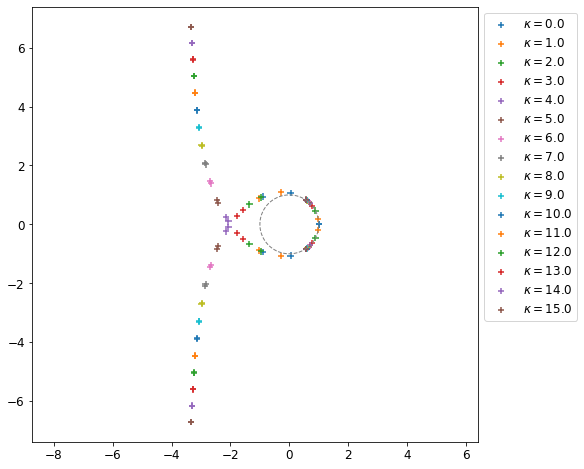
\includegraphics[width=\textwidth]{\localPath/figures/ev_P21.png}
    \caption{Valeurs propres de $P_{2,1}(A)$ pour différentes fréquences $\kappa\in[\![0,15]\!]$.}
    \label{fig:ev:P21}
  \end{subfigure}
  \begin{subfigure}{.5\textwidth}
    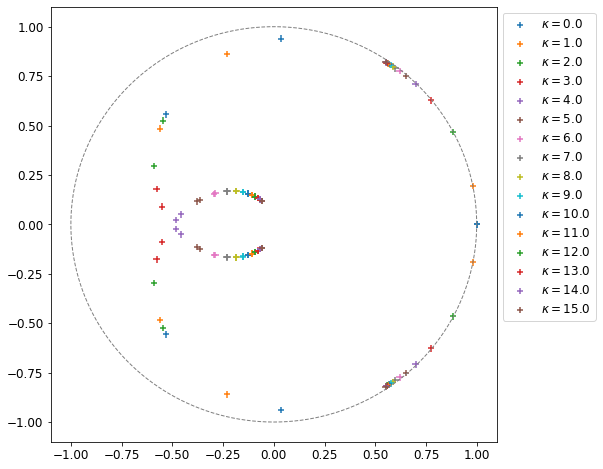
\includegraphics[width=\textwidth]{\localPath/figures/ev_P12.png}
    \caption{Valeurs propres de $P_{1,2}(A)$ pour différentes fréquences $\kappa\in[\![0,15]\!]$.}
    \label{fig:ev:P12}
  \end{subfigure}
  \caption{Valeurs propres de l'approximation de l'exponentielle de $A$ pour différentes fréquences $\kappa\in[\![0,15]\!]$ avec des approximants de Padé où le degré du numérateur et du dénominateur est différent. Les valeurs propres des modes de Fourier négatifs sont obtenues par parité. Les méthodes d'approximation de l'exponentielle de $A$ sont la troncature de Padé d'ordre $(2,1))$ ($P_{2,1}$) à gauche et l'approximant de Padé d'ordre $(1,2)$ ($P_{1,2}$) à droite.}
\end{figure}

%\begin{figure}
%  \centering
%  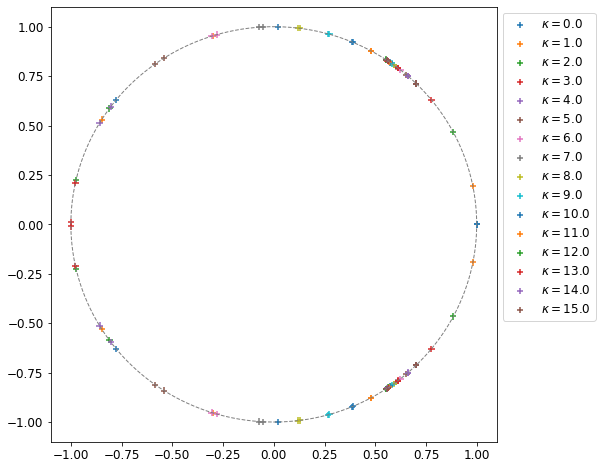
\includegraphics[width=0.5\textwidth]{\localPath/figures/ev_P22.png}
%  \caption{Valeurs propres de $P_{2,2}(A)$ pour différentes fréquences $\kappa\in[\![0,15]\!]$. Les valeurs propres des modes de Fourier négatifs, sont obtenues par parité.}
%  \label{fig:ev:P22}
%\end{figure}

% \begin{figure}
%   \begin{subfigure}{.5\textwidth}
%     \centering
%     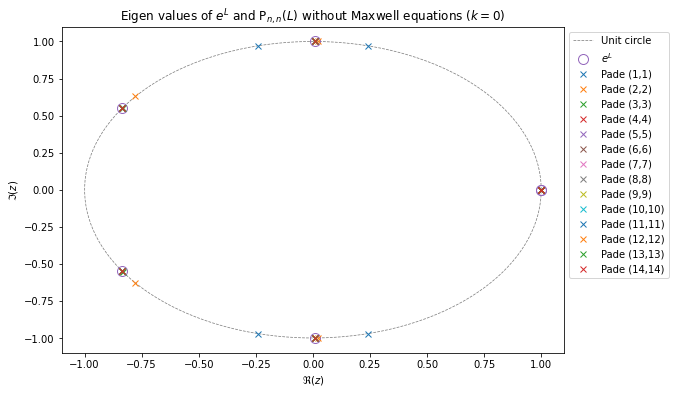
\includegraphics[width=\textwidth]{\localPath/figures/approx_evA0P.png}
%     \caption{Les valeurs propres de $e^{A_0}$ et de $P_{n,n}(A_0)$}
%   \end{subfigure}
%   \begin{subfigure}{.5\textwidth}
%     \centering
%     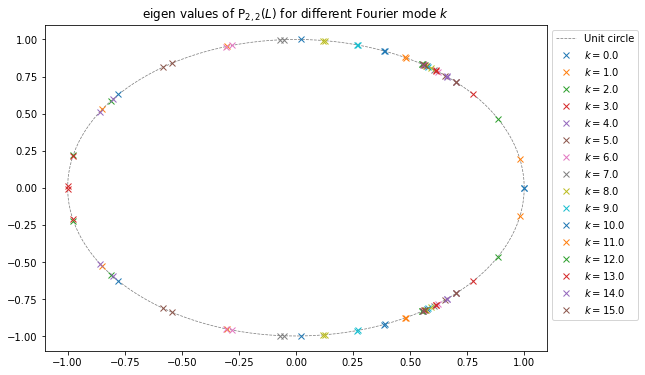
\includegraphics[width=\textwidth]{\localPath/figures/approx_evAkP22.png}
%     \caption{Les valeurs propres de $e^{A}$ et de $P_{2,2}(A)$ pour différentes valeurs de $k\in[\![0,15]\!]$, par symétrie on obtient aussi celles pour $k<0$}
%   \end{subfigure}
%   \caption{Valeurs propres de $e^{A}$ et de $P_{n,n}(A)$ pour $k=0$ (sans les équations de Maxwell) à gauche, et pour différentes valeurs de $k\in[\![0,15]\!]$ à droite.}
%   \label{fig:evAP22}
% \end{figure}

\begin{figure}
  \begin{subfigure}{.5\textwidth}
    \centering
    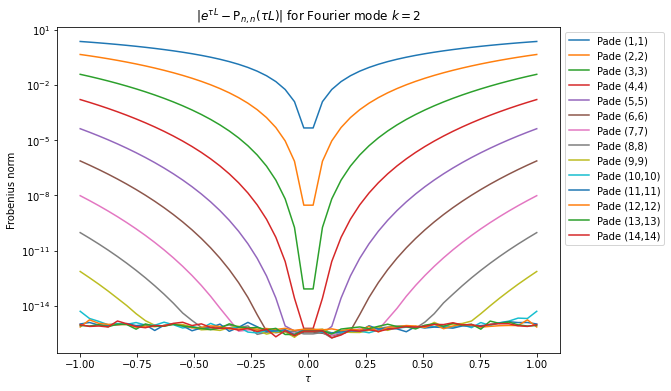
\includegraphics[width=\textwidth]{\localPath/figures/approx_errortA2P.png}
    \caption{L'erreur absolue locale $\|e^{\tau A}-P_{p,p}(\tau A)\|$ pour le mode de Fourier $\kappa=2$}
  \end{subfigure}
  \begin{subfigure}{.5\textwidth}
    \centering
    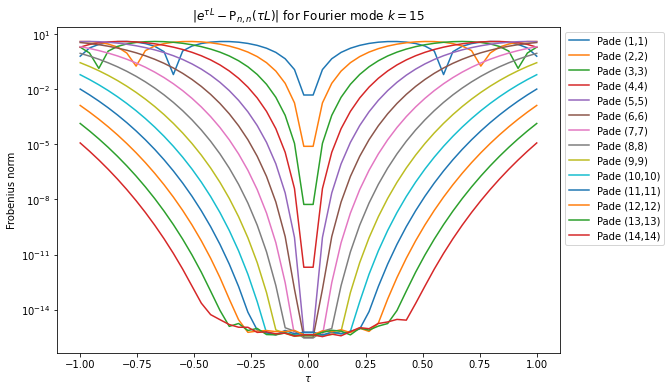
\includegraphics[width=\textwidth]{\localPath/figures/approx_errortA15P.png}
    \caption{L'erreur absolue locale $\|e^{\tau A}-P_{p,p}(\tau A)\|$ pour le mode de Fourier $\kappa=15$}
  \end{subfigure}
  \caption{Erreur absolue locale $\|e^{\tau A}-P_{p,p}(\tau A)\|$ pour deux modes de Fourier $\kappa=2$ à gauche et $\kappa=15$ à droite.}
  \label{fig:pade:error}
\end{figure}

Sur la figure~\ref{fig:pade:error} est tracée l'erreur absolue $\|e^{\tau A}-P_{p,p}(\tau A)\|$ pour deux modes de Fourier $\kappa=2$ à gauche et $\kappa=15$ à droite. On remarque que même pour des hauts modes, l'erreur est limitée par l'erreur machine du calcul numérique pour $p$ suffisamment grand. On observe donc un meilleur comportement que l'approche basée sur la série de Taylor. Ce que l'on confirme par l'étude pour différents modes de Fourier $\kappa$ avec l'approximant de Padé $P_{2,2}$ sur la figure~\ref{fig:pade:error22}.

\begin{figure}
  \centering
  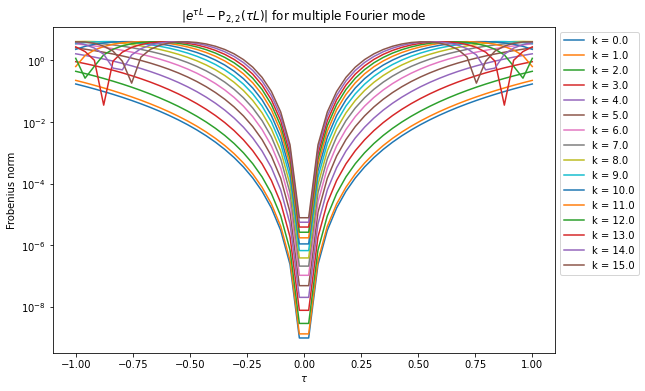
\includegraphics[width=0.75\textwidth]{\localPath/figures/approx_errortAkP22.png}
  \caption{L'erreur absolue locale $\|e^{tA}-P_{2,2}(tA)\|$ pour différents modes de Fourier.}
  \label{fig:pade:error22}
\end{figure}


\subsection{Test sur une advection 2D}
%--------------------------------------------------------------------

Nous souhaitons mettre en place cette stratégie d'approximation de la partie linéaire d'une méthode de Lawson sur une première équation qui nous servira de \emph{toy model} :
$$
  \partial_t u = a\partial_x u + b\partial_y u,\quad u(0,x,y)=u_0(x,y)
$$
où $u(t,x,y)$ est une fonction à valeurs réelles, $(x,y)\in[-2,2]\times[-2,2]$, $t\geq0$, $a,b\in\mathbb{R}$ donnés, et avec des conditions aux bords périodiques en $x$ et $y$. On sait que la solution au temps $t$ est donnée par :
$$
  u(t,x,y) = u_0(x-at,y-bt).
$$
On souhaite résoudre cette équation par une méthode spectrale dans la direction $y$ (partie linéaire de la méthode de Lawson), une méthode WENO5 dans la direction $x$ (partie non-linéaire), et une méthode LRK($s$,$p$) en temps (méthode de Lawson d'ordre $p$ à $s$ étages). Nous obtenons donc l'équation :
$$
  \partial_t \hat{u} = L\hat{u} + N(\hat{u}),\quad u(t=0,x,y) = u_0(x,y)
$$
avec $L = i\kappa b$ et, $N:\hat{u}\mapsto\widehat{a\partial_xu}$. À partir des résultats du chapitre~\ref{chap1}, on peut calculer l'erreur de troncature du schéma en linéarisant la partie non-linéaire :
$$
  u^{n+1} = e^{\Delta tL}\sum_{j=0}^{p}\frac{\Delta t^jN^j}{j!}u^n
$$
On applique le schéma à la solution exacte au temps $t^n$ donnée par $u(t^n)$ :
$$
  \begin{aligned}
    e^{\Delta tL}\sum_{j=0}^{p}\frac{\Delta t^jN^j}{j!}u(t^n) &= e^{\Delta t L}e^{\Delta t N}u(t^n) + \order{\Delta t^{p+1}} \\
      &= e^{\Delta t(L+N)}u(t^n) + \order{\Delta t^{p+1}} \\
      &= u(t^{n+1}) + \order{\Delta t^{p+1}}
  \end{aligned}
$$
On retrouve ainsi l'ordre $p$ de la méthode LRK($s$,$p$). Maintenant en effectuant une méthode d'approximation de l'exponentielle de la partie linéaire $e^{\Delta tL}$, le schéma se réécrit :
$$
  u^{n+1} = \mathfrak{exp}(\Delta tL)\sum_{j=0}^{p}\frac{\Delta t^jN^j}{j!}u^n
$$
où $\mathfrak{exp}$ est la fonction choisie d'approximation de l'exponentielle, c'est-à-dire $\mathfrak{exp}(\Delta tL) = T_m(\Delta tL)$ s'il s'agit de la troncature de la série de Taylor à l'ordre $m$, ou bien $\mathfrak{exp}(\Delta tL) = P_{p,q}(\Delta tL)$ s'il s'agit de l'approximant de Padé d'ordre $(p,q)$ ; dans les deux cas on a bien $\mathfrak{exp}(\Delta tL) = e^{\Delta tL} + \order{\Delta t^{r+1}}$ avec $r = m$ si $\mathfrak{exp}(\Delta tL) = T_m(\Delta tL)$ et $r = p+q$ si $\mathfrak{exp}(\Delta tL) = P_{p,q}(\Delta tL)$. Ainsi :
$$
  \begin{aligned}
    \mathfrak{exp}(\Delta tL)\sum_{j=0}^{p}\frac{\Delta t^jN^j}{j!}u(t^n) &= \left(e^{\Delta t L} + \order{\Delta t^{r+1}}\right)e^{\Delta t N}u(t^n) + \order{\Delta t^{p+1}} \\
      &= e^{\Delta t(L+N)}u(t^n) + \order{\Delta t^{p+1}} + \order{\Delta t^{r+1}} \\
      &= u(t^{n+1}) + \order{\Delta t^{p+1}} + \order{\Delta t^{r+1}}
  \end{aligned}
$$
ce qui nous permet de déterminer l'erreur de troncature du schéma en temps d'une méthode de Lawson LRK($s$,$p$) couplée à une méthode d'approximation de l'exponentielle d'ordre $r$, l'ordre du schéma est $\min(r,p)$.

Il est possible de retrouver ce résultat numériquement en comparant les différentes méthodes et en mesurant l'erreur effectuée pour différentes valeurs de pas de temps $\Delta t$ et ainsi mesurer l'ordre en temps de la méthode. Pour cela on choisit le schéma LRK(3,3) induit par la méthode SSP RK(3,3) de Shu-Osher, on se munit d'une discrétisation spatiale de $243$ points par direction, de plusieurs valeurs de pas de temps $\Delta t\in[0.00158,0.02370]$. La simulation s'effectue jusqu'au temps final $T_f=0.07111$ avec les vitesses $a=1.0$ et $b=0.75$. On regarde l'erreur, par rapport à notre solution de référence en norme 1 :
$$
  e_1 = \| u(T_f,x,y) - u_0(x-aT_f,y-bT_f) \|_1 \approx \sum_{i,j}|u^n_{i,j}-u_0(x_i-aT_f,y_j-bT_f)|\Delta x\Delta y,
$$
ce qui nous permet de tracer, sur la figure~\ref{fig:lrk33ref} l'erreur pour la méthode de référence avec un calcul exact de l'exponentielle de la partie linéaire, ainsi qu'avec une troncature de la série de Taylor d'ordre 4, ordre supérieur à celui de la méthode de Lawson, et un approximant de Padé d'ordre $(2,2)$ (équivalent à un ordre 4), aussi supérieur à l'ordre de la méthode de Lawson, on retrouve bien dans ces cas là l'ordre 3 de la méthode LRK(3,3). La figure~\ref{fig:lrk33taylor} représente l'ordre pour différentes troncatures de la série de Taylor, on remarque que pour des ordres inférieurs à l'ordre de la méthode de Lawson, on retrouve l'ordre de la méthode de Taylor. La figure~\ref{fig:lrk33pade} quant à elle, représente l'ordre pour différents approximants de Padé, on retrouve les mêmes résultats avec une constante d'erreur plus faible.

\begin{figure}
  \centering
  \begin{subfigure}{.45\textwidth}
    \centering
    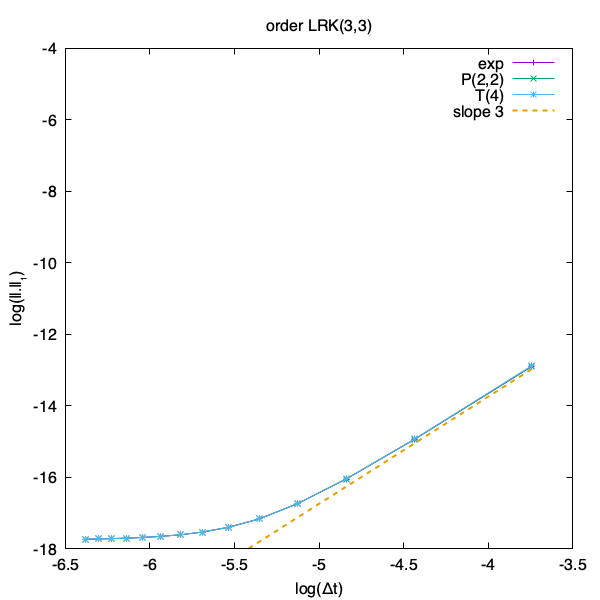
\includegraphics[width=\textwidth]{\localPath/figures/order_lrk33ref.png}
    \caption{Ordre en temps de la méthode LRK(3,3) associée à exponentielle, la série de Taylor d'ordre 4, et l'approximant Padé d'ordre $(2,2)$.}
    \label{fig:lrk33ref}
  \end{subfigure}
  \begin{subfigure}{.45\textwidth}
    \centering
    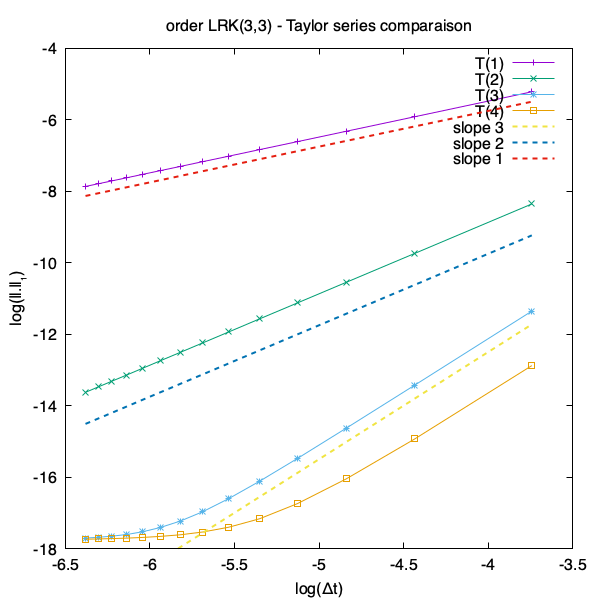
\includegraphics[width=\textwidth]{\localPath/figures/order_lrk33taylor.png}
    \caption{Ordre en temps de la méthode LRK(3,3) associée à la série de Taylor d'ordre 1 à 4.\\ }
    \label{fig:lrk33taylor}
  \end{subfigure}
  \begin{subfigure}{.45\textwidth}
    \centering
    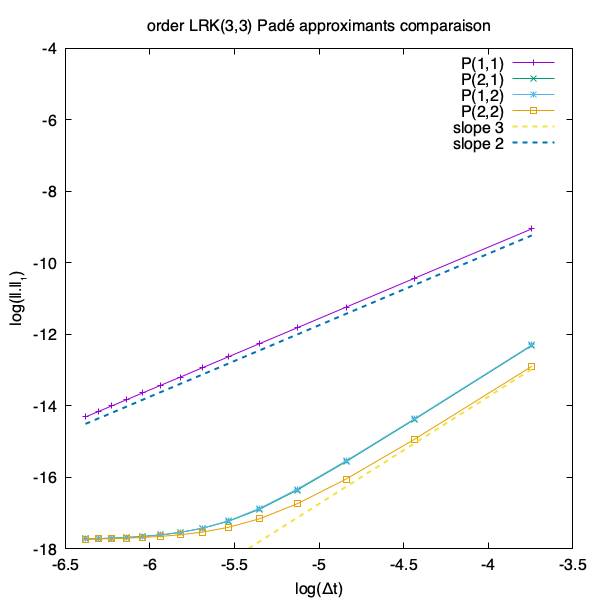
\includegraphics[width=\textwidth]{\localPath/figures/order_lrk33pade.png}
    \caption{Ordre en temps de la méthode LRK(3,3) associée à l'approximant Padé d'ordre $(1,1)$, $(2,1)$, $(1,2)$, et $(2,2)$.}
    \label{fig:lrk33pade}
  \end{subfigure}
  \caption{Ordre en temps de la méthode LRK(3,3) où l'exponentielle de la partie linéaire est approchée par différentes méthodes, série de Taylor ou approximant de Padé de différents ordres. La solution de référence à gauche, le test avec différentes séries de Taylor à droite, et avec différents approximants de Padé en bas.}
  \label{fig:3:order}
\end{figure}

\subsection{Test sur une rotation 2D}
%--------------------------------------------------------------------

Nous poursuivons la mise en place de cette stratégie sur un modèle où les opérateurs dans les directions $x$ et $y$ ne commutent pas, il s'agit du cas d'une rotation à 2 dimensions :
$$
  \partial_t u = -y\partial_x u + x\partial_y u,\quad u(0,x,y)=u_0(x,y)
$$
où $u(t,x,y)$ est une fonction à valeurs réelles, $(x,y)\in[-2,2]\times[-2,2]$, $t\geq0$, $a,b\in\mathbb{R}$ donnés, et avec des conditions aux bords périodiques en $x$ et $y$. Nous souhaitons illustrer le caractère instable de la troncature de Taylor sur un cas simple sans effectuer de calcul d'erreur de troncature, plus compliqué dans le cas non-commutatif. Ainsi nous résolvons de la même manière le problème, c'est-à-dire avec une méthode spectrale dans la direction $y$, et une méthode type différence finie (WENO5) dans la direction $x$. Nous obtenons les résultats présentés sur la figure~\ref{fig:uft3p11} avec comme paramètres $N_x=N_y=81$, le pas de temps $\Delta t=0.020944$, jusqu'au temps final $T_f=1.52891$. La condition initiale est donnée par :
$$
  u_0(x,y) = \exp( -\frac{(x-0.2)^2}{0.25} - \frac{y^2}{0.05} ).
$$
Pour mettre en valeur les instabilités de la méthode de Lawson couplée à une série de Taylor, nous représentons la valeur absolue de la solution. On observe ainsi l'apparition d'instabilités uniquement avec $T_3$ (troncature de la série de Taylor de degré 3), dont l'amplitude est supérieure à 10 pour des hauts modes en $y$, c'est-à-dire les bords du domaine. Aucune instabilité n'est présente lorsque la méthode de Lawson est couplée à un approximant de Padé, ici $P_{1,1}$. Dès que le degré du numérateur est supérieur au dénominateur des instabilités apparaissent, comme nous le verrons par la suite dans la résolution du système de Vlasov-Maxwell.

\begin{figure}
  \centering
  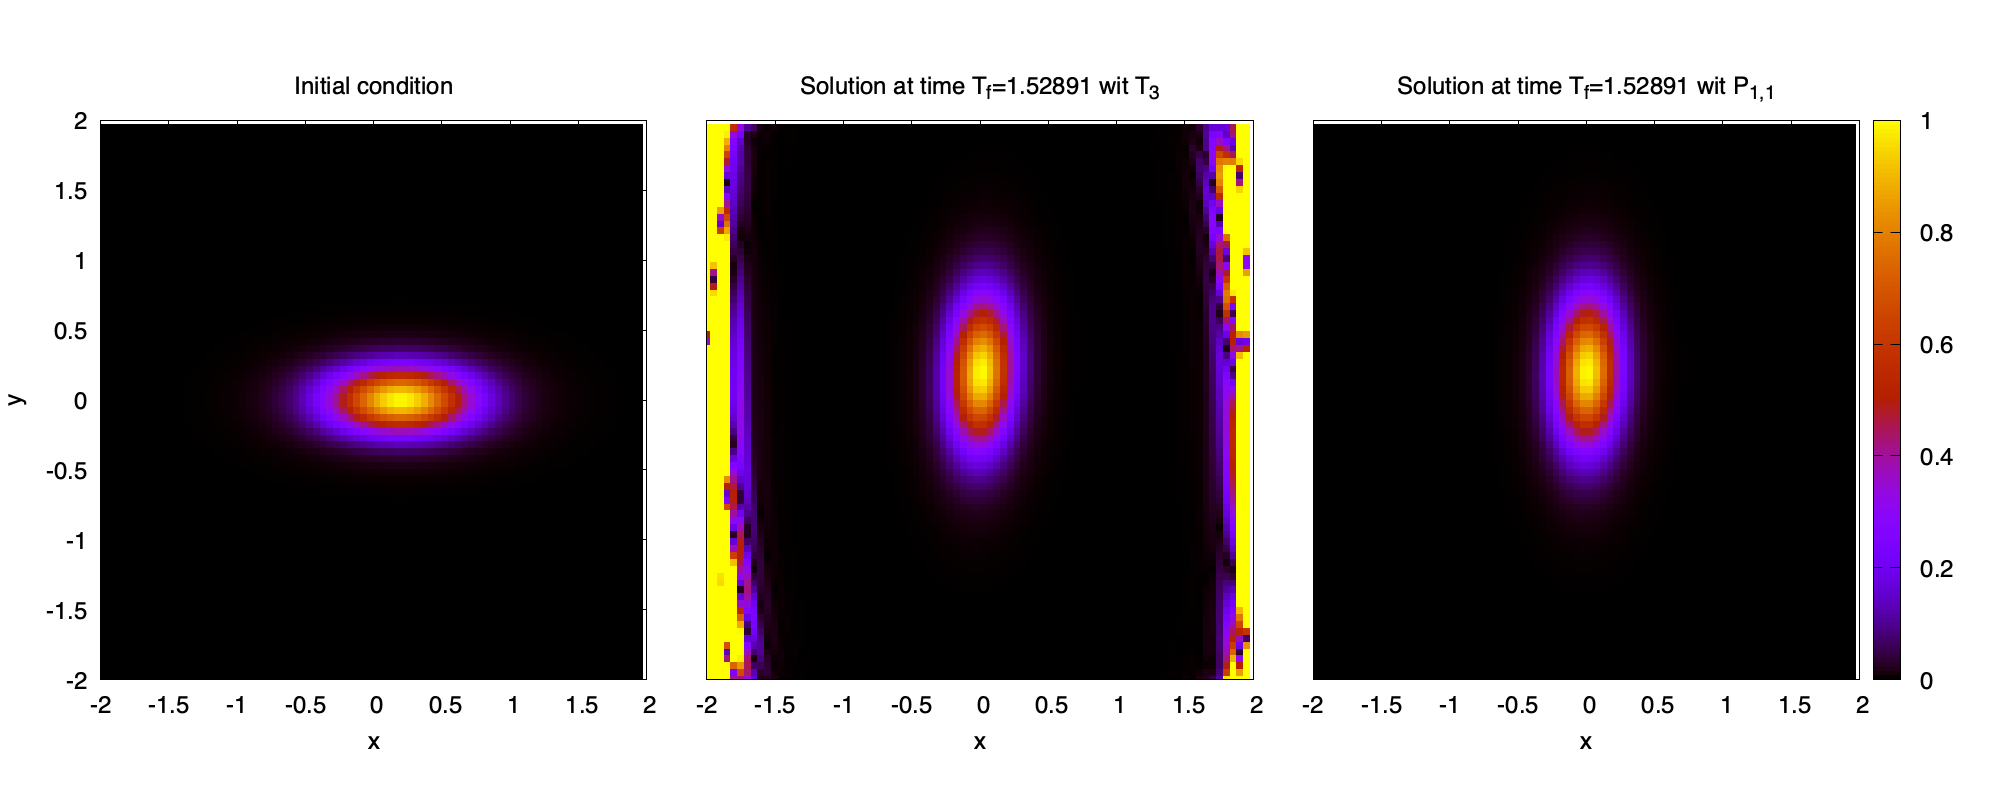
\includegraphics[width=\textwidth]{\localPath/figures/uf_t3p11.png}
    \caption{Solutions de l'équation de rotation 2D avec comme condition initiale une gaussienne (à gauche), et les solutions au temps final $T_f=1.52891$ avec $\Delta t=0.020944$ et $N_x=N_y=81$, données par LRK(3,3) couplé avec $T_3$ (au centre), et couplé avec $P_{1,1}$ (à droite).}
    \label{fig:uft3p11}
\end{figure}

Le calcul d'erreur de troncature a été fait précédemment dans le cas commutatif, il est possible dans le cas non-commutatif de reprendre les calculs effectués dans la section~\ref{ssec:3:cflMaxwell} pour calculer la fonction de stabilité de la méthode $LRK(3,3)$ donnée par la méthode de Shu-Osher :
\begin{equation}
  \begin{aligned}
    u^{n+1} = \Big[ e^{\Delta tL} &+ \Delta t\left(\frac{2}{3}e^{\frac{\Delta t}{2}L}Ne^{\frac{\Delta t}{2}L}+\frac{1}{6}e^{\Delta tL}N + \frac{1}{6}Ne^{\Delta tL}\right) \\
    & + \frac{\Delta t^2}{2}\left(\frac{1}{3}Ne^{\Delta tL}N + \frac{1}{3}e^{\frac{\Delta t}{2}L}Ne^{\frac{\Delta t}{2}L}N + \frac{1}{3} e^{\frac{\Delta t}{2}L}Ne^{-\frac{\Delta t}{2}L}Ne^{\Delta tL} \right) \\
    & + \frac{\Delta t^3}{6}e^{\frac{\Delta t}{2}L}Ne^{-\frac{\Delta t}{2}L}Ne^{\Delta tL}N \Big]u^n
  \end{aligned}
  \label{eq:3:lrk33:nc}
\end{equation}
\newcommand{\R}{R_{\Delta t}^{[L,N]}}
\newcommand{\tR}{\tilde{R}_{\Delta t}^{[L,N]}}
que nous synthétiserons à $u^{n+1}= \R u^n$. Ce schéma vérifie une erreur de troncature d'ordre 3, pour un schéma de Lawson d'ordre $p$ cela se note :
$$
  u(t^{n+1}) - \R u(t^n) = \order{\Delta t^{p+1}}.
$$
Nous cherchons l'erreur de troncature faite par le schéma lorsque la fonction exponentielle est substituée par $\mathfrak{exp}$ ; notons $\tR$ le schéma couplé à la fonction d'approximation de l'exponentielle $\mathfrak{exp}$. On sait que :
$$
  e^{\Delta t L} - \mathfrak{exp}(\Delta tL) = \order{\Delta t^{r+1}},
$$
donc on a :
$$
  \begin{aligned}
    u(t^{n+1}) - \tR u(t^n) &= u(t^{n+1}) - (\tR-\R+\R)u(t^n) \\
                            &= u(t^{n+1}) - \R u(t^n) - (\tR - \R)u(t^n) \\
                            &= \order{\Delta t^{p+1}} - (\tR - \R)u(t^n)
  \end{aligned}
$$
Pour étudier $\tR-\R$, on considère le terme suivant :
$$
  \tau = e^{\frac{\Delta t}{2}L}Ne^{\frac{\Delta t}{2}L} - \mathfrak{exp}\left(\frac{\Delta t}{2}L\right)N\mathfrak{exp}\left(\frac{\Delta t}{2}L\right),
$$
les autres termes se traitant de manière similaire. En utilisant que $e^{\frac{\Delta t}{2}L}-\mathfrak{exp}\left(\frac{\Delta t}{2}L\right) = \order{\Delta t^{r+1}}$, on peut déterminer que :
$$
  \begin{aligned}
    \tau &= \left( e^{\frac{\Delta t}{2}L}-\mathfrak{exp}\left(\frac{\Delta t}{2}L\right)+\mathfrak{exp}\left(\frac{\Delta t}{2}L\right)\right) N \left(e^{\frac{\Delta t}{2}L}-\mathfrak{exp}\left(\frac{\Delta t}{2}L\right)+\mathfrak{exp}\left(\frac{\Delta t}{2}L\right)\right) \\
        & ~~\hphantom{= \big(e^{\frac{\Delta t}{2}L}} - \mathfrak{exp}\left(\frac{\Delta t}{2}L\right)N\mathfrak{exp}\left(\frac{\Delta t}{2}L\right) \\
        &= \left(e^{\frac{\Delta t}{2}L}-\mathfrak{exp}\left(\frac{\Delta t}{2}L\right)\right)N\left(e^{\frac{\Delta t}{2}L}-\mathfrak{exp}\left(\frac{\Delta t}{2}L\right)\right)\\
        & ~~\hphantom{= \big(e^{\frac{\Delta t}{2}L}} + \mathfrak{exp}\left(\frac{\Delta t}{2}L\right)N\left(e^{\frac{\Delta t}{2}L}-\mathfrak{exp}\left(\frac{\Delta t}{2}L\right)\right) + \left(e^{\frac{\Delta t}{2}L}-\mathfrak{exp}\left(\frac{\Delta t}{2}L\right)\right)N\mathfrak{exp}\left(\frac{\Delta t}{2}L\right) \\
        &= \order{\Delta t^{r+1}}.
  \end{aligned}
$$
On obtient ainsi : $e^{\Delta t(L+N)}u(t^n) = u(t^{n+1})+\order{\Delta t^{p+1}}+\order{\Delta t^{r+1}}$ si on décide de coupler le schéma avec une méthode d'approximation de l'exponentielle de la partie linéaire.
